\documentclass{article}
\usepackage[utf8]{inputenc}
\usepackage{tikz}
\usepackage[left=2cm,right=2cm,top=2cm,bottom=2cm]{geometry}

\usetikzlibrary{shapes.geometric, arrows}

\title{Game Spec}
\author{Gaël Berthaud-Müller}
\date{June 2018}


\tikzstyle{startstop} = [rectangle, rounded corners, minimum width=3cm, minimum height=1cm,text centered, draw=black]
\tikzstyle{io} = [trapezium, trapezium left angle=70, trapezium right angle=110, minimum width=3cm, minimum height=1cm, text centered, draw=black, text width=3cm]
\tikzstyle{process} = [rectangle, minimum width=3cm, minimum height=1cm, text centered, draw=black, text width=3cm]
\tikzstyle{decision} = [diamond, minimum width=3cm, minimum height=1cm, text centered, draw=black, aspect=2, text width=3cm]

\tikzstyle{arrow} = [thick,->,>=stealth]
\tikzstyle{arrow} = [thick,->,>=stealth,]
\tikzstyle{line} = [thick,-]


\begin{document}

\maketitle

\newpage
\section{Peers Management}
\subsection{Join process}

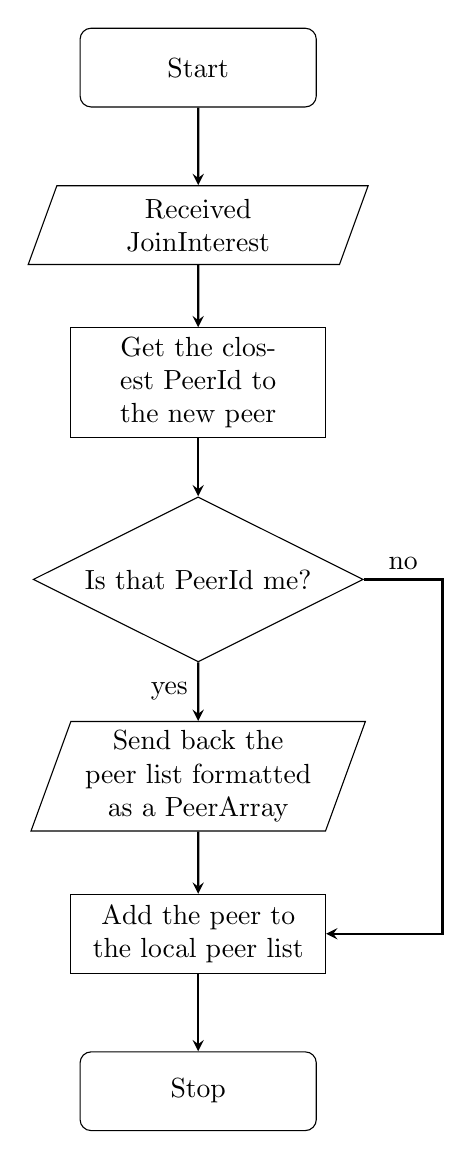
\begin{tikzpicture}[node distance=2cm]

  \node (start) [startstop] {Start};
  \node (in1) [io, below of=start] {Received JoinInterest};
  \node (pro1) [process, below of=in1] {Get the closest PeerId to the new peer};
  \node (dec1) [decision, below of=pro1, yshift=-0.5cm] {Is that PeerId me?};
  \node (out1) [io, below of=dec1, yshift=-0.5cm] {Send back the peer list formatted as a PeerArray};
  \node (pro2) [process, below of=out1] {Add the peer to the local peer list};
  \node (stop) [startstop, below of=pro2] {Stop};

  \draw [arrow] (start) -- (in1);
  \draw [arrow] (in1) -- (pro1);
  \draw [arrow] (pro1) -- (dec1);
  \draw [arrow] (dec1) -- node[anchor=east] {yes} (out1);
  \draw [arrow] (dec1.east) -- node[anchor=south] {no} ++ (1,0) |- (pro2.east);
  \draw [arrow] (out1) -- (pro2);
  \draw [arrow] (pro2) -- (stop);

\end{tikzpicture}

\subsection{Leave process}

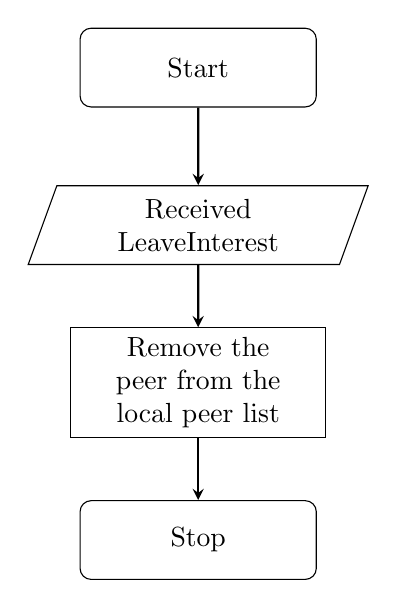
\begin{tikzpicture}[node distance=2cm]
  \node (start) [startstop] {Start};
  \node (in1) [io, below of=start] {Received LeaveInterest};
  \node (pro1) [process, below of=in1] {Remove the peer from the local peer list};
  \node (stop) [startstop, below of=pro1] {Stop};

  \draw [arrow] (start) -- (in1);
  \draw [arrow] (in1) -- (pro1);
  \draw [arrow] (pro1) -- (stop);
\end{tikzpicture}

\section{Objects Management}

\subsection{Becoming coordinator}
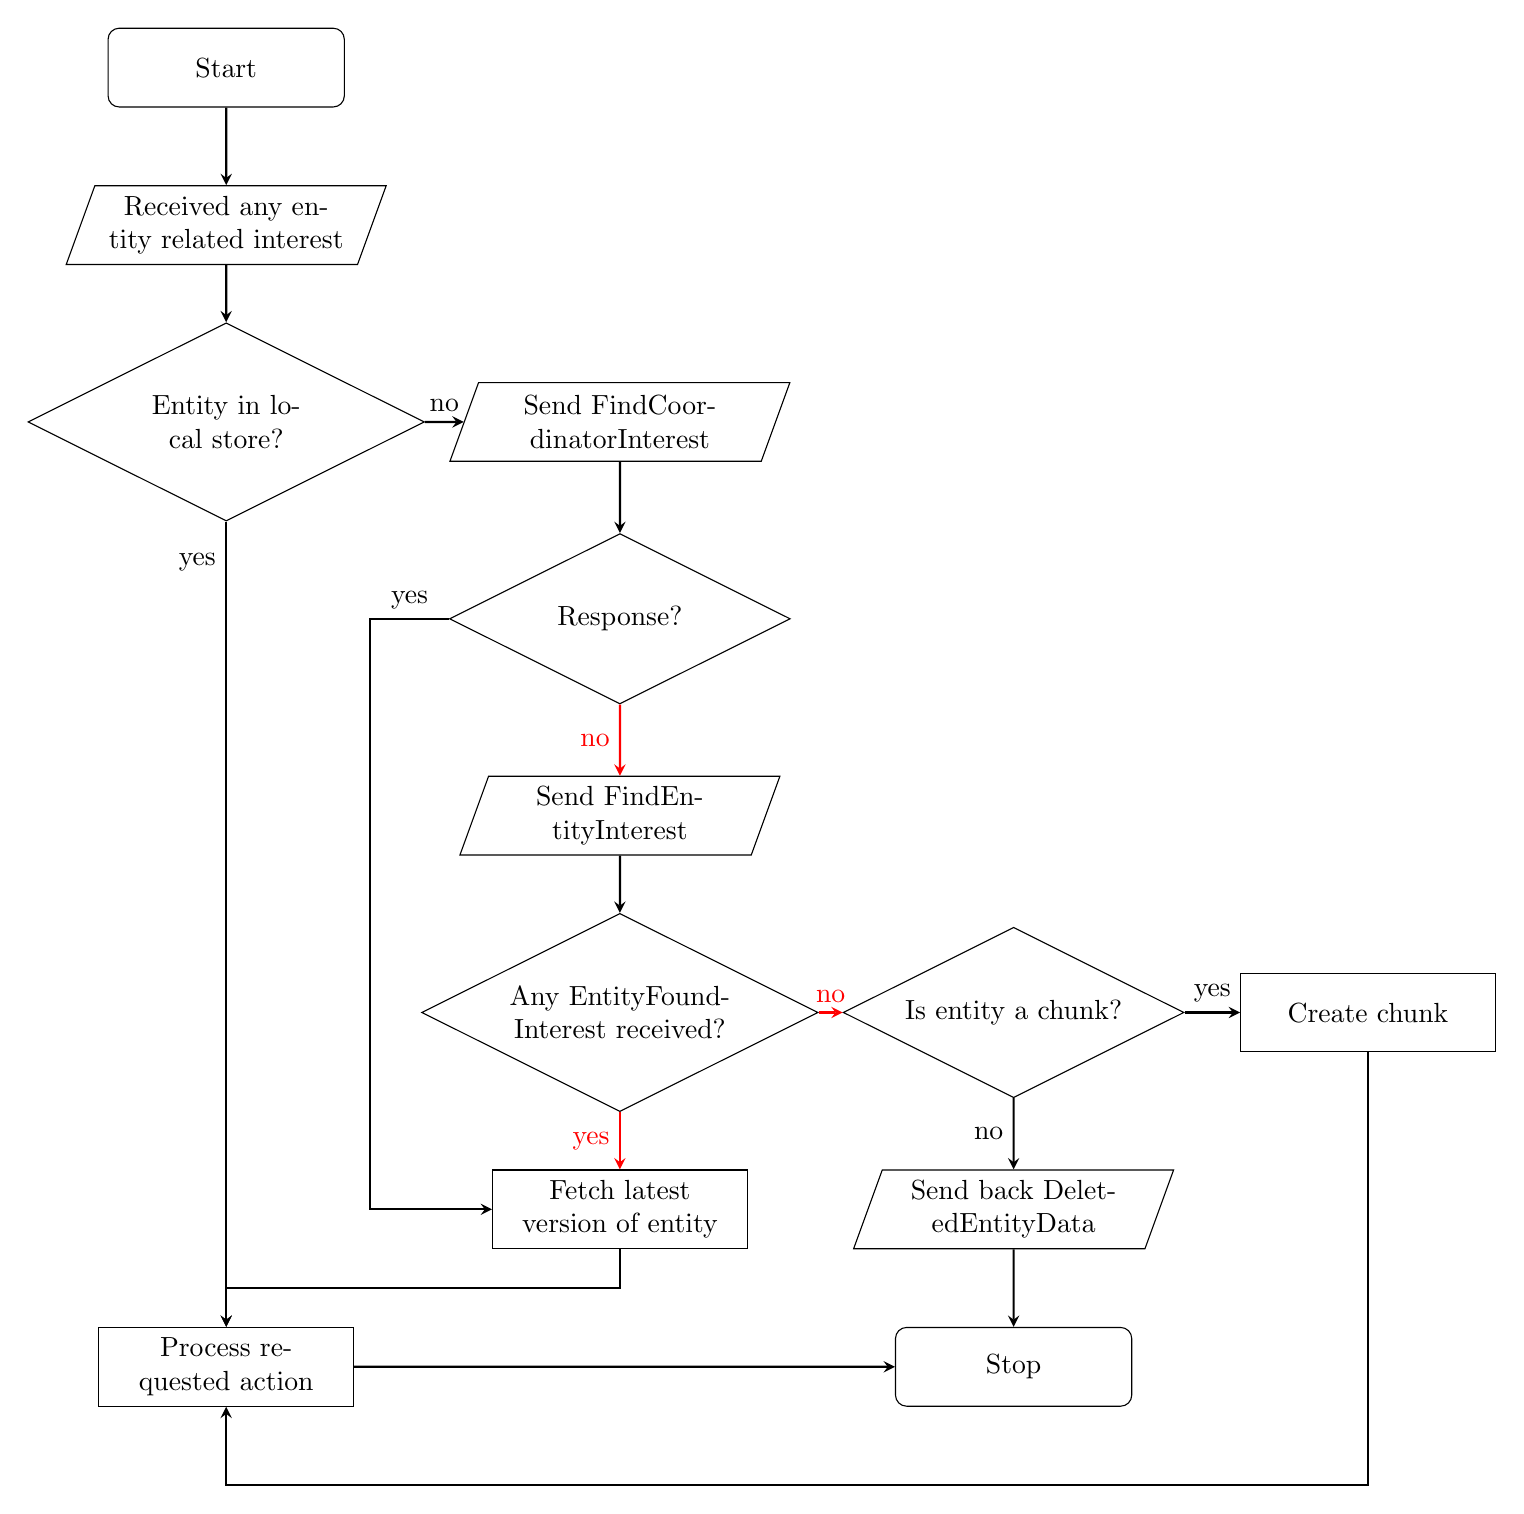
\begin{tikzpicture}[node distance=2cm]
  \node (start) [startstop] {Start};
  \node (in1) [io, below of=start] {Received any entity related interest};
  \node (dec1) [decision, below of=in1, yshift=-0.5cm] {Entity in local store?};

  \node (out1) [io, right of=dec1, xshift=3cm] {Send FindCoordinatorInterest};
  \node (dec2) [decision, below of=out1, yshift=-0.5cm] {Response?};

  \node (out2) [io, below of=dec2, yshift=-0.5cm] {Send FindEntityInterest};
  \node (dec3) [decision, below of=out2, yshift=-0.5cm] {Any EntityFoundInterest received?};
  \node (pro2) [process, below of=dec3, yshift=-0.5cm] {Fetch latest version of entity};

  \node (dec4) [decision, right of=dec3, xshift=3cm] {Is entity a chunk?};
  \node (pro3) [process, right of=dec4, xshift=2.5cm] {Create chunk};
  \node (out3) [io, below of=dec4, yshift=-0.5cm] {Send back DeletedEntityData};

  \node (stop) [startstop, below of=out3] {Stop};
  \node (pro1) [process, below of=dec1, yshift=-10cm] {Process requested action};

  \draw [arrow] (start) -- (in1);
  \draw [arrow] (in1) -- (dec1);
  \draw [arrow] (dec1) -- node[pos=0.05, anchor=east] {yes} (pro1);
  \draw [arrow] (pro1) -- (stop);

  \draw [arrow] (dec1) -- node[anchor=south] {no} (out1);
  \draw [arrow] (out1) -- (dec2);
  \draw [red,arrow] (dec2) -- node[anchor=east] {no} (out2);
  \draw [arrow] (dec2.west) -- node[anchor=south] {yes} ++ (-1,0) |- (pro2);

  \draw [arrow] (out2) -- (dec3);
  \draw [red,arrow] (dec3) -- node[anchor=east] {yes} (pro2);
  \draw [red,arrow] (dec3) -- node[anchor=south] {no} (dec4);
  \draw [arrow] (dec4) -- node[anchor=south] {yes} (pro3);
  \draw [arrow] (dec4) -- node[anchor=east] {no} (out3);

  \draw [arrow] (out3) -- (stop);
  \draw [arrow] (pro3) -- ++ (0,-6) -| (pro1.south);
  \draw [arrow] (pro2)  -- ++ (0,-1) -| (pro1.north);
\end{tikzpicture}
\end{document}
